\clearpage

\section{考察}
\subsection{課題考察}
\begin{enumerate}[1.]
	\item 変圧器の励磁電流について調べ,なぜ流れ,どのような役割をしているのかを考察せよ.\cite{1130282270091029760}
	
	実際の変圧器では,一次・二次巻線には抵抗があるため,負荷電流が流れると銅損が生じる.
	また,鉄心の透磁率は無限大ではないため,磁束$\dot{\phi}$をつくるために電流が必要となる.
	この電流を励磁電流(exciting current)という.
	これによって,鉄心中には鉄損が生じる.
	\item 励磁電流がひずみ波形になる理由を説明せよ.
	
	実際の変圧器では,一次巻線に交流電圧を加えると,鉄心の磁気飽和現象(参考:\ref{hohwa})やヒステリシス現象(参考:\ref{zika})が生じるため,励磁電流は非正弦波交流(ひずみ波形)となる\cite{1130282270091029760}.
	\item 磁性材料のヒステリシス損失について調査せよ.特に使用電圧が変化したとき及び使用電圧の周波数が変化したときについてそれぞれ説明せよ.\cite{11302822718577152}
	\label{hlos}
	
	ヒステリシス損は,鉄心内の磁束が方向及び大きさを変化することにより鉄心を構成する磁気分子が方向・配列を変え,分子相互間に摩擦損が生じることに起因するもの.
	また,ヒステリシスループの囲む面積に比例する.従って,周波数に比例し,さらに,最大磁束$\Phi_{m}$のとき磁束密度$B_{m}$がほぼ$1\,\rm{T}$以下では$B_{m}^{1.6}$に比例し,$1\,\rm{T}$以上では$B_{m}^{2}$に比例する.
	普通,$B_{m}=1 \sim 1.8\,\rm{T}$で使用されるため,鉄心の単位質量当たりのヒステリシス損$\omega_{h}$は以下で与えられる.
	\begin{equation}
		\omega_{h}=\sigma_{h}fB_{m}^{2}=k_{1}\frac{E^{2}}{f}\,[\rm{W/kg}]
		\label{eq:he}
	\end{equation}
	ここで,$\sigma_{h}$はヒステリシス損係数,$f\,[\rm{Hz}]$は周波数,$B_{m}\,[\rm{T}]$は最大磁束$\Phi_{m}$のときの鉄心磁束密度,$k_{1}$は比例定数,$E\,[\rm{V}]$は誘導起電力である.\\
	\weq{he}より使用電圧及び使用電圧の周波数が増加すると損失も増加することがわかる.
	\item 磁性材料のうず電流損について調査せよ.特に使用電圧が変化したとき及び使用電圧の周波数が変化したときについてそれぞれ説明せよ.\cite{11302822718577152}
	\label{uzu}
	
	うず電流損は,磁束の変化によって鉄心内に起電力を生じ,電流が流れる結果,抵抗損失が生じるもので,鋼板の厚さ,周波数及び磁束密度のそれぞれ2乗に比例する.
	これらより,単位重量当たりのうず電流損$\omega_{e}$は次式で与えられる.
	\begin{equation}
	\omega_{e}=\sigma_{e}t^{2}f^{2}B_{m}^{2}=k_{2}t^{2}E^{2}\,[\rm{W/kg}]
	\label{eq:uzue}
	\end{equation}
	ここで,$\sigma_{e}$はうず電流損係数,$t\,[\rm{mm}]$は積層鋼板1枚の厚さ,$k_{2}$は比例定数である.\\
	この\weq{uzue}より使用電圧及び使用電圧の周波数が増加すると損失も増加することがわかる.
	\item 電力計を使用して測定するときの損失とヒステリシス曲線から求めた損失について比較検討し考察せよ.\label{pi}
	
	ヒステリシス損は\ref{hlos}で述べたようにヒステリシスループ内の面積に比例し,\weq{w}を用いて算出することができる.
	なお,ヒステリシスループ内の面積はImageJを用いて算出した.
	また,保存したヒステリシスループの波形は$1\,\rm{DIV}=1\,\rm{cm}$となるように加工をしたため,$[\rm{cm^{2}}]=[\rm{DIV^{2}}]$である.
	\begin{align}
	W_{h}\,[\rm{W}]&=f\times A \times S\times L \times 換算\rm{X}軸測定条件\,[\rm{A/m\cdot 1/DIV}]\times 換算\rm{Y}軸測定条件\,[\rm{Wb/m^{2}\cdot 1/DIV}]\nonumber\\
	\label{eq:w}
	\end{align}
	ここで$A=3.84\times 10^{-4}\,\rm{m^{2}}$は鉄心断面積,$S\,[\rm{cm^{2}}]$は計測したヒステリシスループ内面積,$L=0.122\,\rm{m}$は平均磁路長である.また,実験地は東京であるため$f=50\,\rm{Hz}$である.
	また,$80\,\rm{V}, 100\,\rm{V}$の各場合について測定した損失(\wtab{re1}参照)と\weq{w}を用いて計算により算出した損失を\wtab{los}に示す.
	さらに,測定誤差として$P_{0}$と$W_{h}$の差を求めた.
	
	\begin{table}[h]
	\centering
	\caption{測定損失と計算損失}
	\label{tab:los}
	\begin{tabular}{ccccc}
	\hline
	入力電圧$V\,[\rm{V}]$ & ループ内面積$S\,[\rm{DIV}]$ & 測定損失$P_{0}\,[\rm{W}]$ & 計算損失$W_{h}\,[\rm{W}]$&損失誤差$\,[\rm{W}]$ \\ \hline
	80   & 5.61   & 2.10 & 1.99& 0.11\\
	100  & 8.10   & 3.34 & 2.88 &0.46\\ \hline
	\end{tabular}
	\end{table}
	
	どちらの場合においても測定損失の方が計算損失より大きいことがわかる.
	これは理想の変圧器では考慮していないことがあるからである.(\ref{real}参照)
	
	また,入力電圧が上昇すると損失及び計算値と実際の値の差(誤差)も増えることがわかり,これは上の考察\ref{uzu}, \ref{pi}とも一致する.
	\item 変圧器の鉄心用珪素鋼板について調べよ.\cite{1130282270091060}
	
	変圧器の鉄心には,飽和磁束密度と透磁率が大きく,鉄損の少ない電磁鋼板が用いられる.電磁鋼板は,ヒステリシス損を減少させるためケイ素を$4.5\,\%$程度含有させている.
	電磁鋼板には一方だけ磁束を通しやすい性質の材料もある.また,1枚1枚の電磁鋼板の表面に施してある絶縁皮膜が.温度上昇の一因となるうず電流が流れるのを防ぐ働きをしている.
\end{enumerate}

\subsection{独自考察}
\begin{enumerate}[1.]
	\item 理想変圧器とは以下の条件を満たす変圧器のことをいう\cite{1130000795154912128}.
\begin{itemize}
	\item 巻線の抵抗が0である.
	\item 鉄心の透磁率が無限大であり,したがって磁気回路における磁気抵抗が0である.
	\item 鉄心の鉄損が0である.
	\item 鉄心の磁気飽和は無視できる.
\end{itemize}
\item 一方,実際の変圧器は理想変圧器と異なり,以下のことを考慮しなければならない
\label{real}
\cite{1130154912128}.
\begin{itemize}
	\item 一次及び二次巻線の抵抗や漏れリアクタンスが存在する.
	\item 主磁束を作るために起磁力,すなわち励磁電流が必要である.
	\item 鉄心中に鉄損が存在する.
	\item 鉄心の磁気飽和を無視することは実際上できないが,ここでは特に考慮しない.
\end{itemize}
\item 損失は大きく分けて,コアに発生する鉄損,コイル巻線(誘導機の場合は二次導体も含む)に発生する銅損,そして,摩擦や空気抵抗に起因する機械損に分類できる.
さらに,負荷によって導体,鉄に生じる損失のうち鉄損,銅損に含まれないものを漂遊負荷損と呼ぶ.
これらをまとめたものを\wfig{loss_analysis}に示す.
\begin{figure}[h]
	\centering
	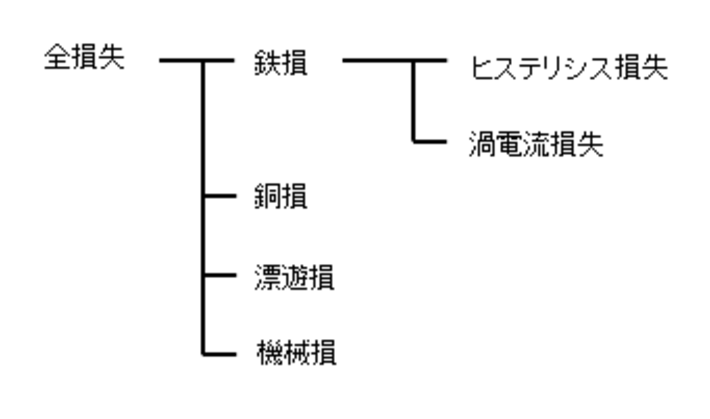
\includegraphics[scale=0.8]{./fig/loss_analysis.pdf}
	\caption{\cite{fdls}}
	\label{fig:loss_analysis}
\end{figure}
\end{enumerate}